\documentclass[varwidth]{standalone}
\usepackage{mwe}
\usepackage[labelfont=normalsize,labelformat=parens,
justification=centering]{caption,subfig} %%% Center the caption
\usepackage{amsfonts,amsmath,amssymb}
\usepackage[slovene]{babel}
\usepackage[utf8]{inputenc}
\usepackage[T1]{fontenc}
  
\usepackage{tikz, verbatim}
\usepackage{pgfplots}
\usetikzlibrary{arrows.meta, calc, positioning, automata}

\newcommand{\subdiv}[3] {
\draw ($ 0.5*#2 + 0.5*#3 $) -- #1;
\draw ($ 0.5*#1 + 0.5*#3 $) -- #2;
\draw ($ 0.5*#1 + 0.5*#2 $) -- #3;
}
\begin{document}
	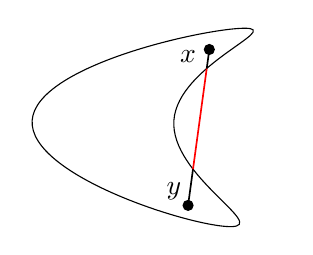
\begin{tikzpicture}[scale=0.9]
		\draw plot [smooth cycle, tension = 1] coordinates {(1, 1.3) (-2, 0) (0.8, -1.5) (0, 0)};
		\begin{scope}
			\clip plot [smooth cycle, tension = 1] coordinates {(1, 1.3) (-2, 0) (0.8, -1.5) (0, 0)};
			\draw[line width= 0.6pt]  (0.5, 1) -- (0.2, -1.2);
		\end{scope}
		\draw[red, line width=0.6pt] ($($(0.5, 1)!.5!((0.2, -1.2)$)!23.8pt!(0.5, 1)$) -- ($($(0.5, 1)!.5!((0.2, -1.2)$)!16.9pt!((0.2, -1.2)$);
		\filldraw (0.5, 1) circle (2pt);
		\filldraw (0.2, -1.2) circle (2pt);
		\draw (0.2, 0.9) node {$x$};
		\draw (0, -1) node {$y$};
	\end{tikzpicture}
\end{document}